\section{Introduction}

The adele class space of \cite{Co-zeta} delivers both a geometric interpretation of the explicit Riemann-Weil formulas as a trace formula, as well as a spectral realization of the zeros of the Riemann zeta function and of $L$-functions with Gr\"ossencharakter. There is a well known analogy, due to Barry Mazur\footnote{on a suggestion of David Mumford},  between knots and primes \cite{Mazur0,Mazur,Mazur1,Mazur2,Morishita,Morishita1}. 
We show that the periodic orbits $C_p$ of length $\log p$ in the Riemann sector $X_\Q:=\Q^\times \backslash \A_\Q/\hatz$ of the adele class space provide a geometric realization of this conjectural relation. 
By construction $X_\Q$ is obtained as the quotient of $\Q^\times \backslash \A_\Q$ by the action of the compact subgroup $\hatz$ of idele classes, acting by multiplication. The space $X_\Q$ admits a simple description in terms of rank one groups \cite{CCas}. Namely, it is the union of the space of such groups, up to isomorphism, and the space of rank one subgroups of $\R$. This latter space is a prototype of  a noncommutative space.\newline
The action of the scaling group $\R_+^*$ on $X_\Q$ gives a Hasse-Weil interpretation of the Riemann zeta function \footnote{completed with its archimedean local factor}  \cite{CC1,ccmonoids} and coincides with the action of the Frobenius automorphisms on the points of the arithmetic site over the tropical semifield $\R_+^{max}$ \cite{CCas}. 
To each prime $p$ corresponds the  periodic orbit $C_p\subset X_\Q$ of length $\log p$ for the action of $\R_+^*$:  $C_p$ consists precisely of  rank one subgroups of $\R$ which are isomorphic to the additive group of the ring $\Z[1/p]$.  We refer to \cite{CCscal1} for the structure of $C_p$ inherited from the scaling site :  $C_p=\R_+^*/p^\Z$ appears as an  elliptic curve in characteristic one,  similar to the Jacobi elliptic curve $\C^*/q^\Z$. The Riemann-Roch formula for $C_p$ involves real valued dimensions. \newline
The role of  the maximal abelian cover $X_\Q^{ab}$ of $X_\Q$ is played by the adele class space $\Q^\times \backslash \A_\Q$ together with the  canonical quotient map $\pi$:
\begin{equation}\label{mappi}
\pi:X_\Q^{ab}:= \Q^\times \backslash \A_\Q\to X_\Q=\Q^\times \backslash \A_\Q/\hatz.
\end{equation}
 Let  $\Z_{(p)}$ be the  ring $\Z$ localized at $p$, $r:\Z_{(p)}\to \F_p$  the residue morphism, and $r^*$ the induced embedding of schemes
\begin{equation}\label{residue}
r^*:\Spec \, \F_p\hookrightarrow \Spec \, \Z_{(p)}.
\end{equation}
Our first result involves the map  $\pi_1^{e t}(r^*)$ at the level of  the \'etale fundamental groups $\pi_1^{e t}$ of schemes. One lets $F r o b_{p}$ be the canonical generator of $\pi_1^{e t}(\Spec\left(\F_p\right))\simeq{\rm Gal}_{}(\bar \F_p/\F_p)$ given by the Frobenius.\newline Theorem \ref{mainglobalintro} shows that the monodromy obtained by lifting the periodic orbit  $C_p$ in the maximal abelian cover $X_\Q^{ab}$ coincides with the multiplication by $r^*\left\{F r o b_{p}\right\}$ in the  abelianized \'etale fundamental group $\pi_1^{e t}(\Spec \, \Z_{(p)})$.
\begin{thm}\label{mainglobalintro} Let $p$ be a prime and $\left\{F r o b_{p}\right\}\in \pi_1^{e t}(\Spec\left(\F_p\right))$ be the canonical generator. The inverse image $\pi^{-1}(C_p)\subset X_\Q^{ab}$ of the periodic orbit $C_p$  is canonically isomorphic to the mapping torus\footnote{in the ordinary topological sense} of the multiplication by $r^*\left\{F r o b_{p}\right\}$  in the abelianized \'etale fundamental group $\pi_1^{e t}(\Spec \, \Z_{(p)})^{ab}$. The canonical isomorphism is equivariant for the action of the idele class group.\end{thm}
 \begin{figure}[H]
\begin{center}
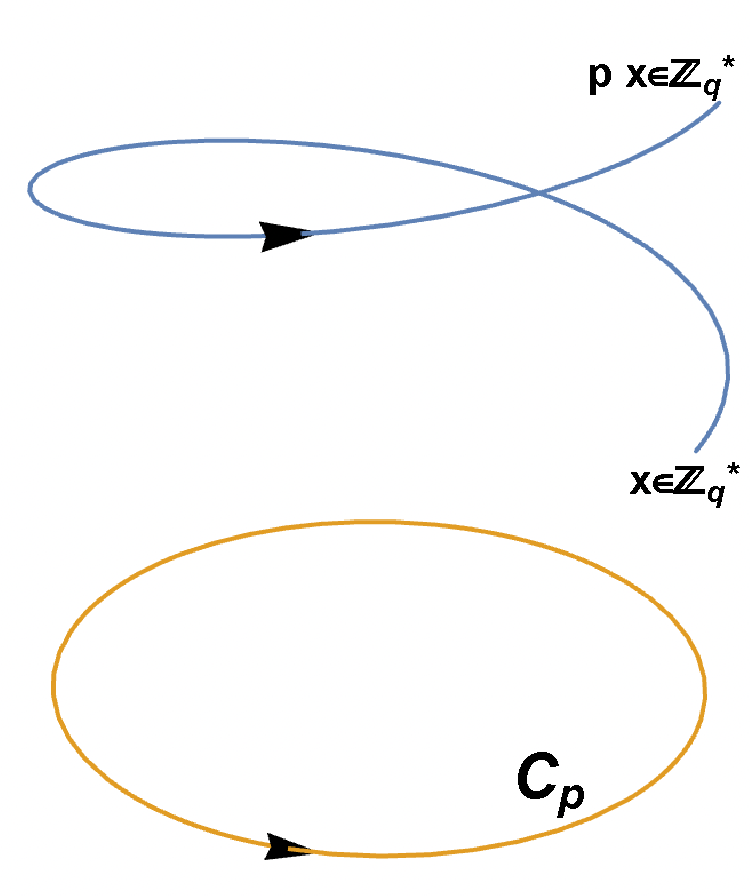
\includegraphics[scale=0.35]{liftknot.pdf}
\end{center}
\caption{Lifting the periodic orbit $C_p$\label{fig1} }
\end{figure}
Our second result gives the geometry underlying the analogy with the linking number of two knots $K,L\subset S^3$ in the three sphere. By definition, the linking number $\operatorname{lk}\left(K, L\right)$ is the monodromy  obtained by lifting the first knot $K$ in the maximal abelian cover $\left(S^3-L\right)^{ab}$ of the complement of the second knot $L$. Equivalently,  $\operatorname{lk}\left(K, L\right)$ is   the image in $\pi_1\left(S^3-L\right)^{a b}\simeq \mathbb{Z}$ of the canonical generator of $\pi_1(K)$
\begin{equation}\label{linking}
\ \ \pi_1(K) \longrightarrow \pi_1\left(S^3-L\right)^{a b}\simeq \mathbb{Z}.
\end{equation}
 In the analogy between knots and primes the role of the knots $K,L$ is played by two distinct primes $p,q$, while the  sphere is replaced by  $\Spec\, \Z$  and  $X_L:=S^3-L$ is replaced by  $\Spec\, \Z[1/q]$.\newline
Given two primes $p\neq q$ we consider the inverse image of the periodic orbit $C_p$ in the semilocal adele class space\footnote{the other places do not play a role}  associated to the set of  places $S=\{ p, q,\infty \}$. The semilocal adele class space is $\Gamma\backslash\left(\Q_p\times \Q_q\times \R\right)$ where $\Gamma:=\{\pm p^mq^n\mid m,n\in \Z\}$. 

\begin{thm}\label{mainintro} The  inverse image  of the periodic orbit $C_p$ in the semilocal adele class space $\Gamma\backslash\left(\Q_p\times \Q_q\times \R\right)$ associated to  $S=\{ p, q,\infty \}$ is the mapping torus of the canonical generator $\left\{F r o b_{p}\right\}$ acting by multiplication in the abelianized \'etale fundamental group  $\pi_1^{e t}(\Spec \, \Z[1/q])^{ab}$ of the complement of $q \in \Spec\, \Z$.	
\end{thm}
Thus  the periodic orbit $C_p$ plays the role of the first knot, and the monodromy of its lift  in the maximal abelian cover of the complement of $q \in \Spec\, \Z$ is the element $p\in \Z_q^*$. In the analogy between knots and primes developed in \cite{Mazur,Morishita,Morishita1}, $p\in \Z_q^*$  plays the role of the linking number\footnote{and allows one to compare the quadratic reciprocity with the antisymmetry of the linking number} of $p$ with $q$.\newline
Section \ref{sect3} provides a detailed description of the natural stratification of the semilocal adele class space $\A_{\Q,S}=\Gamma\backslash\left(\Q_p\times \Q_q\times \R\right)$ that generates a spectral sequence for the $K$-theory of the associated $C^*$-algebras.\newline
Finally, section \ref{sect4} describes the canonical 
 codimension one foliation of the three dimensional manifold $\Gamma\backslash\left(\A_{\Q,S}\times \underline{E \Gamma}\right) =\Gamma\backslash\left(\Q_p\times \Q_q\times \R \times \R^2\right)$   source of the Baum-Connes map \cite{BC} which computes   the $K$-theory of the $C^*$-algebra $\cA=C_0(\A_{\Q,S})\rtimes \Gamma$.


